% Chapter 1

\chapter{Visualization} % Main chapter title

\label{Chapter3} % For referencing the chapter elsewhere, use \ref{Chapter1} 

\lhead{Chapter 3. \emph{Visualization}} % This is for the header on each page - perhaps a shortened title

%----------------------------------------------------------------------------------------

\section{Variable Distributions and Patterns }

\subsection{Numerical Variable Distributions:}
For numerical variables like 'Unit price,' 'Quantity,' 'Tax 5\%,' 'Total,' etc., their distributions can be visualized using histograms. Histograms show how the values are spread across different ranges or bins. Important aspects to consider include:
Central Tendency: Is the distribution centered around a particular value (mean or median)?
Spread: How spread out are the values? Are there outliers?
Shape: Does the distribution have a particular shape, such as normal, skewed, or bimodal?

\subsection{Categorical Variable Distributions}
For categorical variables like 'Branch,' 'City,' 'Customer type,' 'Payment,' etc., their distributions can be visualized using count plots or bar charts. These plots show the frequency of each category. Important considerations include:
{\begin{itemize}
    \item Frequency: Which categories are most common or rare?
    \item Imbalances: Are there significant imbalances in the distribution of categories?
\end{itemize}}
Frequency: Which categories are most common or rare?
    \item Imbalances: Are there significant imbalances in the distribution of categories?

\subsection{Bivariate Relationships}
Exploring relationships between variables, especially between numerical and categorical variables, helps understand how variables interact. Box plots, pair plots, or other bivariate visualizations provide insights into how the distribution of a numerical variable varies across different categories of a categorical variable.

\subsection{Time Trends}
For temporal variables like 'Date' in a time series dataset, understanding the distribution involves looking at how values change over time. Time series plots can reveal trends, seasonality, or patterns in the data.


% ---------------------------------------------------------------------------------------------------------

\section{Why is Visualization required here?} 
Visualizations are a cornerstone of data exploration and communication. They play a crucial role in this project by doing the following.

\subsection{Unveiling Hidden Patterns and Relationships}
\begin{itemize}
\item Revealing trends, correlations, and anomalies that might be obscured in raw data tables.
\item Exposing patterns in customer behavior, product preferences, sales patterns, and seasonal influences.
\item Highlighting relationships between variables, such as the impact of promotions on sales or the influence of customer demographics on purchasing habits.
\end{itemize}


\subsection{Enhancing Understanding and Communication}
\begin{itemize}

\item Transforming complex data into intuitive and accessible visual representations. 
\item Making insights easier to comprehend, interpret, and share among stakeholders with varying levels of technical expertise.
\item Fostering collaboration and discussion by providing a visual platform for exploration and debate.
\end{itemize}

\subsection{Guiding Further Analysis and Decision-Making:}
\begin{itemize}

\item Informing subsequent steps in the data mining process, such as feature selection, model building, and evaluation.
\item Supporting data-driven decision-making by providing evidence-based insights for marketing strategies, inventory management, customer segmentation, and other business initiatives.	

\end{itemize}
% --------------------------------------------------------------------------------------------------

\section{Visualizations }

\begin{figure}[h]
    \centering
    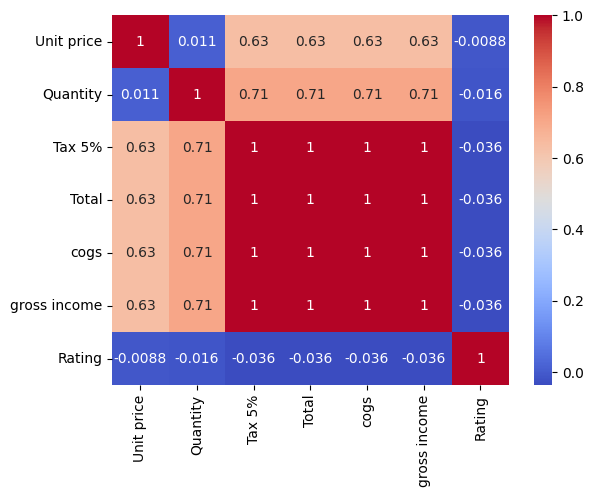
\includegraphics[width=0.7\textwidth]{Chapters/ch3/ch_3_heatmap.png}
    \caption{Correlation Matrix Heatmap}
    % \label{fig:example}
\end{figure}

Features like Tax, Total, Cost of Goods Sold, and Gross Income, can be seen having maximum positive correlation- which means they are highly directly correlated. Most other features are also highly correlated in a positive manner. Rating is slightly negatively correlated with all other features.

\begin{figure}[h]
    \centering
    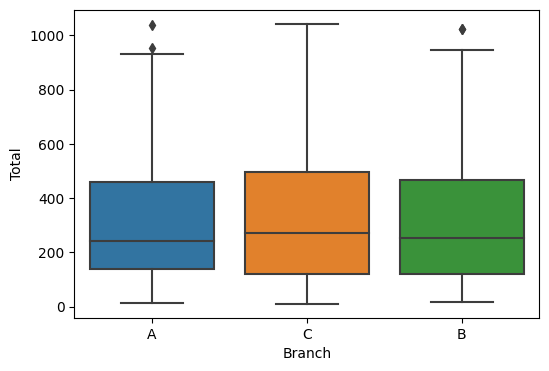
\includegraphics[width=0.7\textwidth]{Chapters/ch3/ch_3_boxplot.png}
    \caption{Box plot by branch}
    % \label{fig:example}
\end{figure}
The distribution of the ‘Total’ column by Branch can be observed here. All Branches seem to have a higher distribution of values for ‘Total’ from the 50th to 75th percentile (middle to Q3). This means that all branches have higher totals per average transaction. How high though? As can be seen from the boxplots, the trend of higher distribution of values starts from around the \$200 mark. 

\begin{figure}[h]
    \centering
    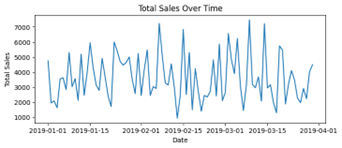
\includegraphics[width=0.7\textwidth]{Chapters/ch3/tim_s_1.png}
    \caption{Time series graph}
    % \label{fig:example}
\end{figure}
The plot reveals the overall trend of total sales across all three branches over time. It allows us to identify seasonal patterns in sales, such as fluctuations due to holidays or periods of high demand. It reveals higher trends in sales patterns, such as in mid-February and mid-March, that could indicate significant events or changes in store operations.

\begin{figure}[h]
    \centering
    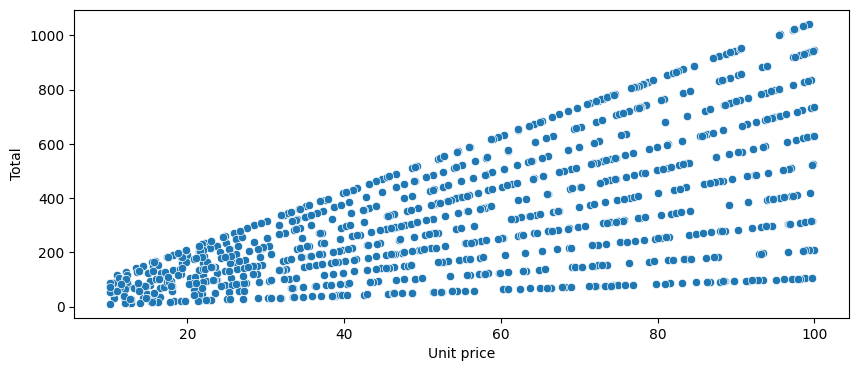
\includegraphics[width=0.7\textwidth]{Chapters/ch3/ch_3_scatterplot.png}
    \caption{Scatter plot}
    % \label{fig:example}
\end{figure}
Each point represents a single transaction, positioned according to its unit price and total value. Here we can observe a clear positive correlation, as values for ‘Total’ tend to increase with ‘Unit Price’. Not only this, but the density of points (transactions) also sees an upward trend as both features increase in their respective magnitudes.

\begin{figure}[h]
    \centering
    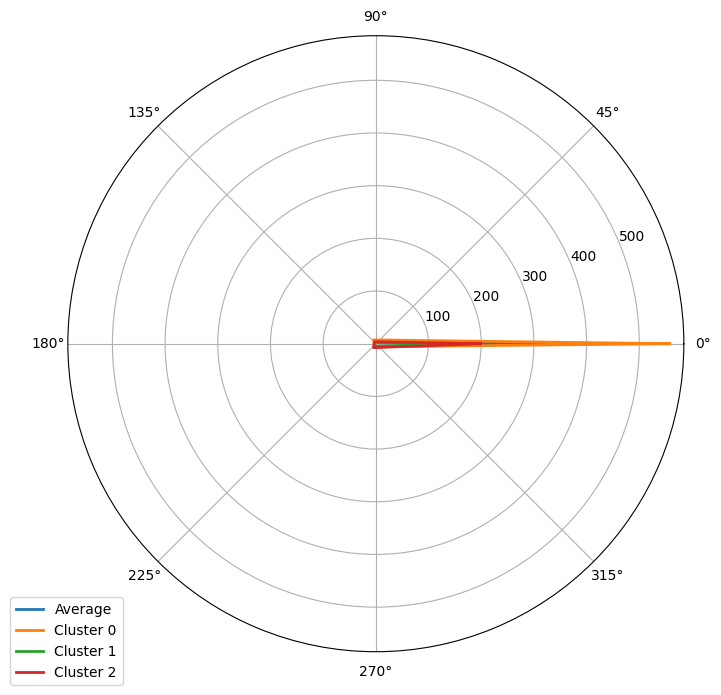
\includegraphics[width=0.7\textwidth]{Chapters/ch3/ch_3_spiral.png}
    \caption{Radar graph}
    % \label{fig:example}
\end{figure}
\newpage
To make this, I selected specific features ('Total', 'Quantity', 'Rating') for segmentation. After this I standardized the features and then using K-Means, performed clustering (3 clusters). Each cluster represents a group of transactions with similar characteristics in terms of these variables. This helps identify distinct segments or groups within the data, allowing for a more nuanced understanding of how certain features contribute to the segmentation. Cluster 0 (represented by the outermost line in orange) covers most of the radar chart, occupying about 2/5ths of the outermost line. This suggests that a significant portion of the 3 features fall into Cluster 0. Cluster 1 is visible as a green segment for about 1/5th of the outer line. This indicates that there is a distinct group of data points (transactions) in Cluster 1 with specific characteristics that differentiate them from other clusters. Similarly, Cluster 2 is represented by a red segment for about 1/5th of the outer line. This suggests another distinctive group of data points with different characteristics compared to the rest of the dataset. The dominance of Cluster 0 suggests that it has a larger influence on the overall dataset. The cyclical appearance of different colored segments may indicate temporal patterns in customer behavior.

\begin{figure}[h]
    \centering
    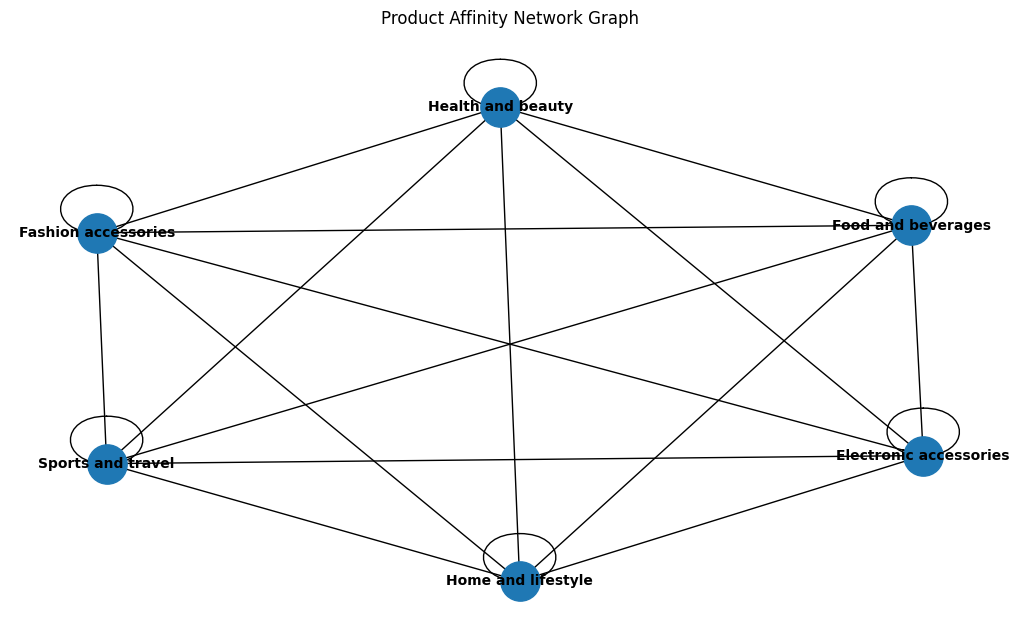
\includegraphics[width=0.7\textwidth]{Chapters/ch3/ch_3_graph.png}
    \caption{Product affinity network graph}
    % \label{fig:example}
\end{figure}
\newpage
An undirected graph G is created using nx.Graph(). This graph represents relationships between products. The pairs of products represent the sequence of products in the 'Product line' column. Edges are added to the graph (G) using \verb|G.add_edges_from(pairs)|. Each pair of consecutive products in the 'Product line' forms an edge in the graph. The graph helps identify which products are often purchased together or follow each other in sales transactions. Each node here is connected to every other node which suggests a high level of interconnectedness. In the context of product affinity, it implies a strong association between all pairs of product lines. Hence, there are no specific clusters or groups of product lines; rather, all product lines are somewhat related to each other.



